% ch01 Introduction (书页 1–9 / 分册p015–p023)
% 第1章 Introduction
\chapter{绪论}

固体物理学脱胎于量子力学对固体中电子导电问题的应用。这个看似简单的问题曾令人束手无策，因为晶格每个格点上离子的存在似乎构成了导电的明显障碍。于是，电子如何避开离子就成了基本问题。尽管这一问题的答案早已众所周知，它仍不失为阐明固体物理精髓的一个绝佳例证：多者之中自有组织。每个电子都调整自己的波长，以利用晶格的周期性。在没有杂质时，导电是完美的。因此，理解了“周期性蕴含完美导电”这一简单事实之后，人们便清楚地认识到：金属中实验观测到的电阻率并非来自电子撞上一个个离子，而是来自污垢（无序）、由离子动力性运动传递的热效应，或电子–电子相互作用。本书将逐一考察这些效应，着眼于找出隐藏在背后、能使这类相互作用的物理得以简化的组织原则。

\section{自发对称性破缺}

寻找有助于简化多体系统物理的组织原则，是现代固体物理——更一般地说，凝聚态物理——的核心课题。对称性便是这样一种工具。考虑初等量子力学课程中通常讲授的置换对称性（permutation symmetry）这一简单例子。这一对称性是海森堡（W. Heisenberg）在全同粒子不可分辨性的背景下引入量子力学的。置换群的元素数目有限，因而对应于一种分立对称性。置换对称性使我们能够把基本粒子分成两类：玻色子在两个粒子互换下为偶，费米子为奇。正如我们将在分数量子霍尔效应的语境中看到的，这一对称性还可以推广为：两个粒子互换时出现非整数的相位。

在很大程度上，凝聚态系统中最切题的对称性通常是连续的，例如转动对称性。自发破缺一个连续对称性会带来一个基本的后果。例如，固体中声子的存在或磁体中自旋波的存在，都源于连续对称性的自发破缺。所谓自发，意指不施加外场。晶体中离子的周期性排列破坏了连续的平移对称性和转动对称性。仅凭晶格的存在而实现的这种连续对称性自发破缺，必然伴随一种无质量、无自旋的玻色型激发。这类被称为南部–戈德斯通玻色子（Nambu–Goldstone bosons）的无质量无自旋玻色子（文献 [G1961; N1960]）必然伴随连续对称性的破缺而出现，这一点不难从下面的考察中推出。我们考虑一个具有拉格朗日量
\begin{equation*}
\mathcal{L}=T-V(\phi),
\tag{1.1}
\end{equation*}
的系统，它由动能 $T$ 和势能 $V(\phi)$ 组成，其中我们允许 $\phi$ 为复函数。所谓该系统在对称操作下不变，可用下式表达：
\begin{equation*}
V(\phi)=V(\phi+\epsilon\delta\phi),
\tag{1.2}
\end{equation*}
其中 $\epsilon\delta\phi$ 是对称操作的生成元（generator）。这里 $\epsilon$ 是无穷小量。我们暂时假定 $\delta\phi$ 与空间无关。为说明这一恒等式的含义，考虑形如 $V(\phi)=\epsilon_0|\phi|^2$ 的势。该势在 $\phi\to\phi\mathrm{e}^{\mathrm{i}\theta}$ 型的变换下不变。令 $\theta$ 为完全与空间无关的小量，则我们可以展开指数并只保留一阶项。于是 $\phi\to\phi(1+\mathrm{i}\theta)$，我们把 $\epsilon\delta\phi$ 认作 $\mathrm{i}\theta\phi$；也就是说，$\epsilon=\theta$，$\delta\phi=\mathrm{i}\phi$。这一对称性即 $\mathrm{U}(1)$ 对称性，存在于保持电荷守恒的模型之中。把 $V(\phi)$ 按 $\epsilon$ 展开到线性阶便意味着，只要对称性完好无损，就有
\begin{equation*}
\delta\phi\,\frac{\delta V}{\delta\phi}=0,
\tag{1.3}
\end{equation*}
现在明确假定对称性被破缺，使 $V\to V(\phi_0+\chi)$，其中 $\phi_0$ 使势取极小，而 $\chi$ 不能像式 (1.2) 中那样写成某个对称操作的生成元。既然势有一个极小，作如下展开便是合理的：
\begin{equation*}
V(\phi_0+\chi)=V(\phi_0)+\frac{1}{2}\chi^2\left.\frac{\partial^2 V}{\partial\phi^2}\right|_{\phi=\phi_0}=V(\phi_0)+\frac{1}{2}\chi^2 m^2,
\tag{1.4}
\end{equation*}
即到二阶恢复项处截断。第二项可用于在标准简谐展开中定义质量 $m$；由于我们是围绕极小点展开的，这一项天然是半正定的。有了这个方程在手，我们把式 (1.3) 对 $\phi$ 求微商：
\begin{equation*}
\frac{\partial\,\delta\phi}{\partial\phi}\,\frac{\delta V}{\delta\phi}+\delta\phi\,\frac{\partial^2 V}{\partial\phi^2}=0,
\tag{1.5}
\end{equation*}
第一项在极小点处取值为零，这意味着
\begin{equation*}
\delta\phi\,\left.\frac{\partial^2 V}{\partial\phi^2}\right|_{\phi=\phi_0}=0
\tag{1.6}
\end{equation*}
在破缺对称态中对 $\phi$ 的任何变动都必须恒等地成立。由于 $\delta\phi$ 非零，式 (1.6) 仅当二阶导数项为零——等价地，$m^2=0$——时才能成立。也就是说，质量为零。这就是戈德斯通定理（Goldstone's theorem，文献 [G1961]）。连续对称性被破缺的每一个生成元，都对应存在一个零模。由于这一定理，对称性在物理学的所有领域——特别是粒子物理和凝聚态物理——都占据着核心地位。凝聚态系统中出现的无质量玻色子通常代表整个多体系统的集体激发。在流体中，声子是纯纵向的，源于伽利略不变性的自发破缺。在固体中，声子既有横波也有纵波，但它们与伽利略、平移和转动对称性的自发破缺之间并无简单的对应关系。在磁体中，自旋波即磁振子（magnon）是从转动对称性的自发破缺中产生的无能隙集体激发。

当然，我们可以放宽 $\theta$ 与空间无关的约束。这样一来，我们便能考察在局域变换而非整体变换（$\theta$ 与空间无关）之下会发生什么。我们对势能的分析保持不变，但动能
\begin{equation*}
T\to\frac{1}{2}(\partial_\mu\phi^*)(\partial^\mu\phi)+\frac{1}{2}|\phi|^2(\partial_\mu\theta(x))^2,
\tag{1.7}
\end{equation*}
确实获得了一个描述相位空间变化的新项。如果 $\mathrm{U}(1)$ 对称性不被这一变换破坏，那么第二项就必须为零。要求
\begin{equation*}
\partial_\mu\theta=0
\tag{1.8}
\end{equation*}
成立，就意味着 $\theta$ 必须空间均匀，对称性才能得以保持。于是，连续 $\mathrm{U}(1)$ 对称性破缺的一个后果是 $\theta$ 必须空间不均匀。超导体中正是这种情形。事实上，超导体内部的电流完全来自相位的空间变化；只要把 $\psi$ 解读为超导态的波函数，即 $\psi=\Delta\mathrm{e}^{\mathrm{i}\theta}$，这一点便可从电流的量子力学方程
\begin{equation*}
j_\mu=\frac{\mathrm{e}\hbar}{m}\,\mathrm{Im}\,\psi^\dagger\partial_\mu\psi=\frac{\mathrm{e}^*\hbar}{m}|\Delta|^2\partial_\mu\theta,
\tag{1.9}
\end{equation*}
看出。在超导性那一章里，我们将确切地看到这种局面是如何出现的。我们将把 $\psi$ 解读为超导态的序参量（order parameter）。虽然巴丁–库珀–施里弗（Bardeen–Cooper–Schrieffer，BCS）超导理论在建立时肯定没有被表述为连续对称性破缺的一个例子，但这正是该理论所依据的基本原理。事实上，超导电性的关键要素——电荷为 $2e$ 的载流子与超流（supercurrent）——全都源自 $\mathrm{U}(1)$ 对称性的破缺。

从破缺对称性中应运而生的无质量玻色子，通常会催生意想不到的新物理。例如，声子传递电子之间的配对，从而在诸如 Hg 这样的金属以及更复杂的体系（例如 MgB$_2$）中引发超导电性。然而，这类南部–戈德斯通玻色子能以何种方式影响任何系统，受到严格规则的支配。正如阿德勒（Adler）所指出的（文献 [A1965]），由连续对称性破缺产生的无质量玻色子所诱导的相互作用，必须与转移动量成正比。更正式地说，经由交换南部–戈德斯通玻色子而传递的相互作用，只能以导数耦合（derivative coupling）的方式出现。因此，交换动量为零时，相互作用为零。这一原理意味着，在元素超导体中传递配对的电子–声子相互作用本质上是动力学的。我们将在电子–声子耦合的语境中，通过一个显式推导来验证这一重要原理。于是，完全从晶格的存在出发，声子以及它们所传递的相互作用的类型便可以容易地推出。

\section{跟踪破缺的对称性：序参量}

序参量的思想是凝聚态物理中另一个强有力的概念。序参量跟踪破缺的对称性：也就是说，它们在对称破缺相中非零，否则为零。考虑一个铁磁体。局域地看，每个自旋都可以指向任意方向；这正是高温下没有任何对称性被破坏时的情形。在由热涨落控制的相变中，通常具有较高对称性的是高温相。为定量刻画自旋集合中的有序程度，我们把每个自旋算符的 $z$ 分量求和，
\begin{equation*}
M=\frac{1}{N}\sum_i\langle S_i^z\rangle,
\tag{1.10}
\end{equation*}
再除以自旋数目 $N$。这里 $S_i^z$ 是格点 $i$ 上原子的自旋的 $z$ 分量，尖括号表示对系统诸态的热平均。$M$ 就是磁化强度。高温下、任何对称性尚未破缺时，磁化强度恒为零。在足够低的温度下，自旋有序化，磁化强度取得非零值。以铁为例，其居里温度即有序化温度为 1340 K。结果发现，在磁化温度以下，一整块铁的大部分区域磁化强度为零。出现这种局面是因为磁化强度一般是空间的函数，于是一块铁并不能均匀地破坏对称性。事实上，块体磁体中的实际磁化并不是自发获得的，而是通过某种外部手段把所有各个磁畴排列一致而获得的。在磁畴边界处，磁化强度改变符号，形成畴壁（domain wall）。铁中典型的畴尺度约为 300 个离子。把一块铁放入磁场，会使所有磁畴取向到同一方向；即使在外场撤去很久之后，这种局面仍会持续。这一点很重要，因为重新取向后的磁畴态并不构成系统的最小能量态。磁畴靠被钉扎在缺陷上而锁定就位。于是可以预期：当磁化场变化时，磁化强度不会连续地改变，而是随着畴壁从缺陷处脱钉，以不连续跳变的方式改变。这正是巴克豪森（Barkhausen；原文误拼作 Barkhaussen）效应的实质——磁化强度在外磁场中出现的微小不连续跳变；它归根结底也是铁磁体磁化曲线呈现图 1.1 所示磁滞的原因。

\begin{figure}[H]\centering
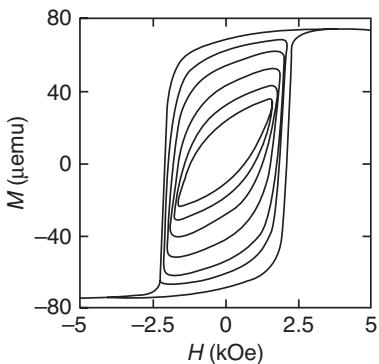
\includegraphics[width=0.5\textwidth]{figs/ch01/fig_1.1.jpg}
\caption*{图 1.1\quad CoPtCrB 薄膜的磁化强度随外加场变化的磁滞回线。多层 Co/Pt 结构被用于存储器存储。转载自文献 Carpenter et al., Phys. Rev. B 72, 052410 (2005)。}\label{fig:auto:1.1}
\end{figure}

也就是说，把场加上再撤去是一个路径依赖的过程，取决于哪些磁畴先后脱钉。

在磁性系统中至关重要的是，每个自旋在局域上有两个自由度。高温下两个态都可以实现；温度足够低时，自旋态之一被选中。这种态的选择性可以用形如
\begin{equation*}
V(M)=-\frac{1}{2}\alpha M^2+\frac{1}{4}\gamma M^4,
\tag{1.11}
\end{equation*}
的双阱势（double-well potential）来建模，其中 $M$ 是磁化强度，$\alpha$ 和 $\gamma$ 为正。该势的极小出现在
\begin{equation*}
M_\pm=\pm\sqrt{\frac{\alpha}{\gamma}}.
\tag{1.12}
\end{equation*}
高温下两个极小都可以实现，因而磁化不可能出现。我们取 $\alpha>0$，保证了 $M$ 偏离 $M_\pm$ 需要付出能量。结果，$V$ 的最小能量不是零，而是非零值 $V_0=-\alpha^2/4\gamma$。照现在这个样子，我们的理论在变换 $M\to-M$ 下是完全对称的。可以肯定，如果我们把标量场 $M$ 平移一个常数、使 $M\to M_++\phi(x)$，从而重新表述我们的理论，物理不应有任何改变。新的势
\begin{equation*}
V'=V_0+\left(-\frac{1}{2}\alpha+\frac{3}{2}\gamma M_+^2\right)\phi^2+\gamma M_+\phi^3+\frac{1}{4}\gamma\phi^4
\tag{1.13}
\end{equation*}
在新场 $\phi$ 的表述下不再显出对称性。为什么？我们在 $V$ 的某个极小附近展开，实际上是把对称性隐藏了起来。本质上，我们通过把磁化强度取为 $M_+$ 而破坏了对称性。在对称破缺相中，自旋向上与向下不再等价。场 $M$ 起着磁有序之度量的作用。$M$ 就是序参量。旧势在 $M$ 取非零值时达到极小；与此不同，$V'$ 的极小出现在 $\phi(x)=0$ 处。这对应于真真空。在铁磁体的经典模型中，磁化强度连续地开启，
\begin{equation*}
M\propto|T-T_{\mathrm{c}}|^{\alpha},
\tag{1.14}
\end{equation*}
发生在非零温度 $T_{\mathrm{c}}$ 处；它在 $T=0$ 时取得最大值。指数 $\alpha$ 是序参量开启的临界指数。

\begin{figure}[H]\centering
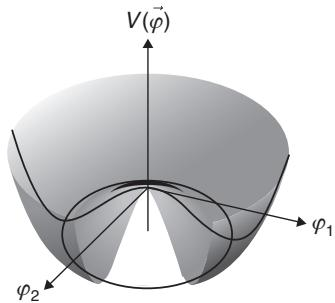
\includegraphics[width=0.5\textwidth]{figs/ch01/fig_1.2.jpg}
\caption*{图 1.2\quad 复标量场 $\varphi$ 对应的势。极小对应于满足 $\varphi_1^2+\varphi_2^2=\alpha/\gamma$ 的圆。}\label{fig:auto:1.2}
\end{figure}

当我们把势修改为
\begin{equation*}
V(\varphi)=-\alpha\varphi^*\varphi+\gamma(\varphi^*\varphi)^2,
\tag{1.15}
\end{equation*}
以允许复标量场 $\varphi=\frac{1}{\sqrt{2}}(\varphi_1+\mathrm{i}\varphi_2)$ 时，便出现一个稍复杂一些的破缺对称性例子。对 $\alpha>0$ 与 $\gamma>0$，该势绘于图 1.2。相应的拉格朗日量取如下形式：
\begin{equation*}
\mathcal{L}=\frac{1}{2}(\partial_\mu\varphi^*)(\partial^\mu\varphi)-\left(\alpha\varphi^*\varphi+\gamma(\varphi^*\varphi)^2\right).
\tag{1.16}
\end{equation*}
我们的拉格朗日量具有整体对称性 $\varphi\to\varphi\mathrm{e}^{\mathrm{i}\theta}$，其中 $\theta$ 是常数。由于这一对称性，$V$ 的极小现在取满足 $\varphi_1^2+\varphi_2^2=\alpha/\gamma$ 的一整圈值，如图 1.2 所示。也就是说，连续整体对称性的结果是存在无穷多个鞍点。与前面磁化强度的单标量场情形一样，我们可以通过定义 $\varphi=(\sqrt{\alpha/\gamma}+f(x)+\mathrm{i}g(x))$ 来围绕这圈极小展开。也就是说，我们用手动的方式破坏了对称性。由于在极小处 $\varphi_1$ 与 $\varphi_2$ 并不独立，这一变换并不是分别对 $\varphi_1$ 和 $\varphi_2$ 的简单平移。结果，二次项实质上只有一个自由度。我们可以把这一点解读为其中一个标量场的质量消失，这与戈德斯通定理——连续对称性破缺必然导致一个无质量模式出现——是一致的。复场取得非零值的这种解，正是超导转变的核心。巴丁–库珀–施里弗解所澄清的是：用复序参量在超导态中取得非零值来表述的朗道–金兹堡（Landau–Ginzburg）唯象处理，在电子–声子相互作用中有其微观基础。这样的相互作用传递配对，超导态的序参量是配对形成振幅与 $\mathrm{e}^{\mathrm{i}\theta(r)}$ 的乘积，其中 $\theta$ 是对场（pair field）的相位。

\begin{figure}[H]\centering
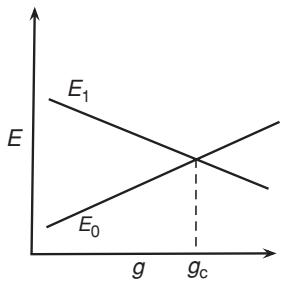
\includegraphics[width=0.45\textwidth]{figs/ch01/fig_1.3.jpg}
\caption*{图 1.3\quad 基态 $E_0$ 和第一激发态 $E_1$ 作为耦合常数 $g$ 的函数的能级图。在 $g_{\mathrm{c}}$ 处的交叉标志着基态与第一激发态之间的相变。}\label{fig:auto:1.3}
\end{figure}

我们关于低温相通常对称性较低的论断，只在经典范围内成立。有许多 $T=0$ 下的对称性破缺例子与热涨落毫无关系。这类相变受真空涨落即不确定性原理的支配。一般地说，这类相变的实现方式仅仅是改变系统的某个参量，就能使多体系统的各量子力学态之间发生转变。考虑一个哈密顿量 $H(g)$，其中 $g$ 是耦合常数。该系统作为 $g$ 函数的典型能级图绘于图 1.3。如果作为 $g$ 的函数，第一激发态与基态相交，就会发生向第一激发态的相变。要使这一转变连续，必须有 $\partial E/\partial g=0$。这类情形将在第 14 章中明确讨论。

\section{超越破缺对称性}

尽管对称性在给集体现象分类时非常有用，物理学中仍然充满了这样的例子：物质诸态之间的转变，双方具有相同的对称性，却依然截然不同。一个明显的例子是液–气转变，或分数量子霍尔态的形成。然而，我们在此着重关注的、最能代表强耦合物理的例子，是那些以某种束缚态（bound state）的形成为标志特征的转变。例如考虑橡胶中的硫化（vulcanization）或交联（crosslinking）转变。在未硫化态，橡胶是一种粘性液体，其中的长链单体（monomer）各自独立运动。相邻单体间的交联导致形成一个高度缠结、相互嵌套的无定形态（amorphous state），这就定义了硫化转变。虽然单体在硫化态中是局域化的，但它们的位置是无规的，因此不存在布拉格峰。尽管如此，我们仍可定义一个恰当的序参量（文献 [GCZ1996]），它反映如下事实：在 $t=0$ 与 $t=\infty$ 这两个时刻，液体中单体链的构型彼此不同，而在无定形态中它基本上保持静止。橡胶由此获得的回弹力与涌现出来的静态模量，都源于单体被有效地黏合在一起。在高能物理中，介子即夸克的束缚态，是原子核中低能下传播的自由度。它们的出现并未破坏任何连续对称性。在与本书关系更密切的问题中，非磁性基质中的一个磁性杂质在低于某一特征温度时与所有传导电子形成束缚态，同样不破坏任何对称性，甚至不引发相变。这种束缚态的形成正是近藤问题（Kondo problem）的精髓；近藤问题堪称重正化群（renormalization group）原理最关键的胜利之一。正如我们将通过系统地积分掉高能自由度所证明的，束缚态之所以出现，是因为杂质与基质电子之间的耦合常数发生发散。因此，在低温下把磁性自由度与传导电子自由度分开来考虑是不正确的。在低能下涌现出一个初始的紫外（UV）完备拉格朗日量中并不存在的新实体——这是强耦合体系的标志性特征。虽然强耦合下出现的这些新自由度在弱耦合或高温区域并不存在，但两个态仍然是绝热相连（adiabatically connected）的：通过改变系统参数，我们可以从一个相平滑地走到另一个相。尽管如此，两个相截然不同。它们拥有不同的自由度，而且不存在以单一实体来统一描述这类系统的理论。束缚态的形成是强耦合物理中的标准范式；我们将看到，莫特问题——部分填充能带中的绝缘态——也不例外。

另一个关键例子是费米液体理论（Fermi liquid theory）。这一理论的首要信条是：金属的激发态与无相互作用电子气的激发态一一对应。金属中的相互作用当然不为零。然而，它们受到强烈屏蔽，基本上可以按短程相互作用来处理。朗道（文献 [L1957]）的论断是：所有这类短程排斥相互作用都不会破坏无相互作用电子气中电子激发的锐利性。这种局面竟能成立，或许要算大自然最非凡的原理之一。为什么短程相互作用在金属中可以被忽略？答案在于一个基本的重正化原理，我们将在第 12 章中给出。解决任何多体问题的关键，是辨认出真正传播的自由度。在相互作用电子气中断言传播自由度就是色散关系为 $p^2/2m$ 的单个电子，这极不平凡。事实上，这一点无法直接从哈密顿量推出，还需要一个进一步的事实。这个进一步的事实就是费米面的存在。我们将看到，让费米液体理论得以奏效的基本原理是：费米面对短程排斥相互作用异常顽强。我们将明确证明，源于这类相互作用的所有重正化（文献 [P1992; SM1991; BG1990]）都朝向费米面。结果，这类相互作用可以被有效地积分掉，留下的是缀饰电子（dressed electrons）即准粒子，从而印证了朗道的核心信条（文献 [L1957]）：金属的低能电子激发谱与无相互作用费米气体的激发谱完全相同。因此，在维数大于等于 2 时破坏费米液体理论，是出了名的困难。在一维空间中，正如我们将看到的，相互作用总是相关的（relevant），于是出现了一种新的物质状态，称为卢廷格液体（Luttinger liquid），其中自旋和电荷都在运动，但速度不同。在更高维数下，这个问题尚无定论，堪称固体物理中最关键的悬而未决的问题。

费米液体理论之所以使超导态的 BCS 理论成为可能，在于它干净利落地辨认出了传播自由度；同样地，要弄清在铜氧化物高温超导体中是什么配对起来形成超导凝聚体，就必须对其正常态中的传播自由度作出类似的辨认。这个问题格外困难，因为母体材料全都是反铁磁莫特绝缘体。关于这一非凡问题的一些已有共识的物理，以及一种前瞻性的视角，将在本书最后一章讨论。

\section*{参考文献}
\addcontentsline{toc}{section}{参考文献}
\begin{itemize}[leftmargin=2em,itemsep=0pt,parsep=0pt,label={}]
\item {[}A1965] S. L. Adler, Phys. Rev. B 137, 1022 (1965); Phys. Rev. 139, B 1638 (1965).
\item {[}BG1990] G. Benefatto and G. Gallavotti, J. Stat. Phys. 59, 541 (1990).
\item {[}GCZ1996] P. M. Goldbart, H. E. Castillo, A. Zippelius, Adv. Phys. 45, 393 (1996).
\item {[}G1961] J. Goldstone, Nuovo Cimento 19, 154 (1961).
\item {[}N1960] Y. Nambu, Phys. Rev. 117, 648 (1960).
\item {[}L1957] L. D. Landau, Sov. Phys. JETP 3, 920 (1957); 5, 101 (1957); 8 70 (1959).
\item {[}P1992] J. Polchinski, arXiv:hep-th/9210046.
\item {[}SM1991] R. Shankar, Physica A177, 530 (1991).
\end{itemize}
